% DO NOT COMPILE THIS FILE DIRECTLY!
% This is included by the other .tex files.

\begin{frame}
\titlepage
\end{frame}

\begin{frame}
  \frametitle{The aim of this presentation}
  \begin{itemize}
    \item MISP Project
    \begin{itemize}
     \item What has happened since the last MUG
     \item Give you a brief update over the highlights
     \item Ongoing rework
    \end{itemize}
    \item Cerebrate
    \begin{itemize}
     \item Update on Cerebrate
    \end{itemize}
  \end{itemize}
\end{frame}

\begin{frame}
\frametitle{MISP update}
\begin{center}

\includegraphics[scale=0.3]{images/misp.png}
\end{center}
\end{frame}

\section{What has happened since the last MUG}

\begin{frame}
  \frametitle{Statistics}
  \begin{itemize}
    \item Since the last MISP summit (16/11/2022) we've had:
    \begin{itemize}
        \item {\bf 6} releases
        \item {\bf 871} commits
        \item {\bf 40} contributors contributing to the core software and its components
        \item {\bf 102} pull-requests on MISP components (MISP objects, taxonomies, galaxy, modules, warning-lists)
    \end{itemize}
  \end{itemize}
\end{frame}

\section{Give you a brief update over the highlights}

\begin{frame}
  \frametitle{A topical listing of the new major features}
  \begin{itemize}
      \item {\bf Workflow} improvements
      \item {\bf STIX 2.1} improvements along with TAXII integration
      \item {\bf Freetext} import modernisation
      \item {\bf Logging} and {\bf security} improvements
      \item {\bf Dashboard} rework
      \item {\bf Security fixes} and other improvements
  \end{itemize}
\end{frame}


\begin{frame}
  \frametitle{Workflows}
  \begin{itemize}
     \item Continuous ongoing work
     \item Further addition of {\bf logic nodes} for more advanced {\bf branching} decision trees
     \item Additional {\bf action nodes} (such as e-mailing improvements)
     \item The inclusion of new {\bf triggers} based on community feedback
     \item {\bf Filtered data} paths within workflows (e.g. Only execute this set of actions on a subset of the workflow's input data)
  \end{itemize}
\end{frame}

\begin{frame}
\frametitle{Workflows}
\begin{center}
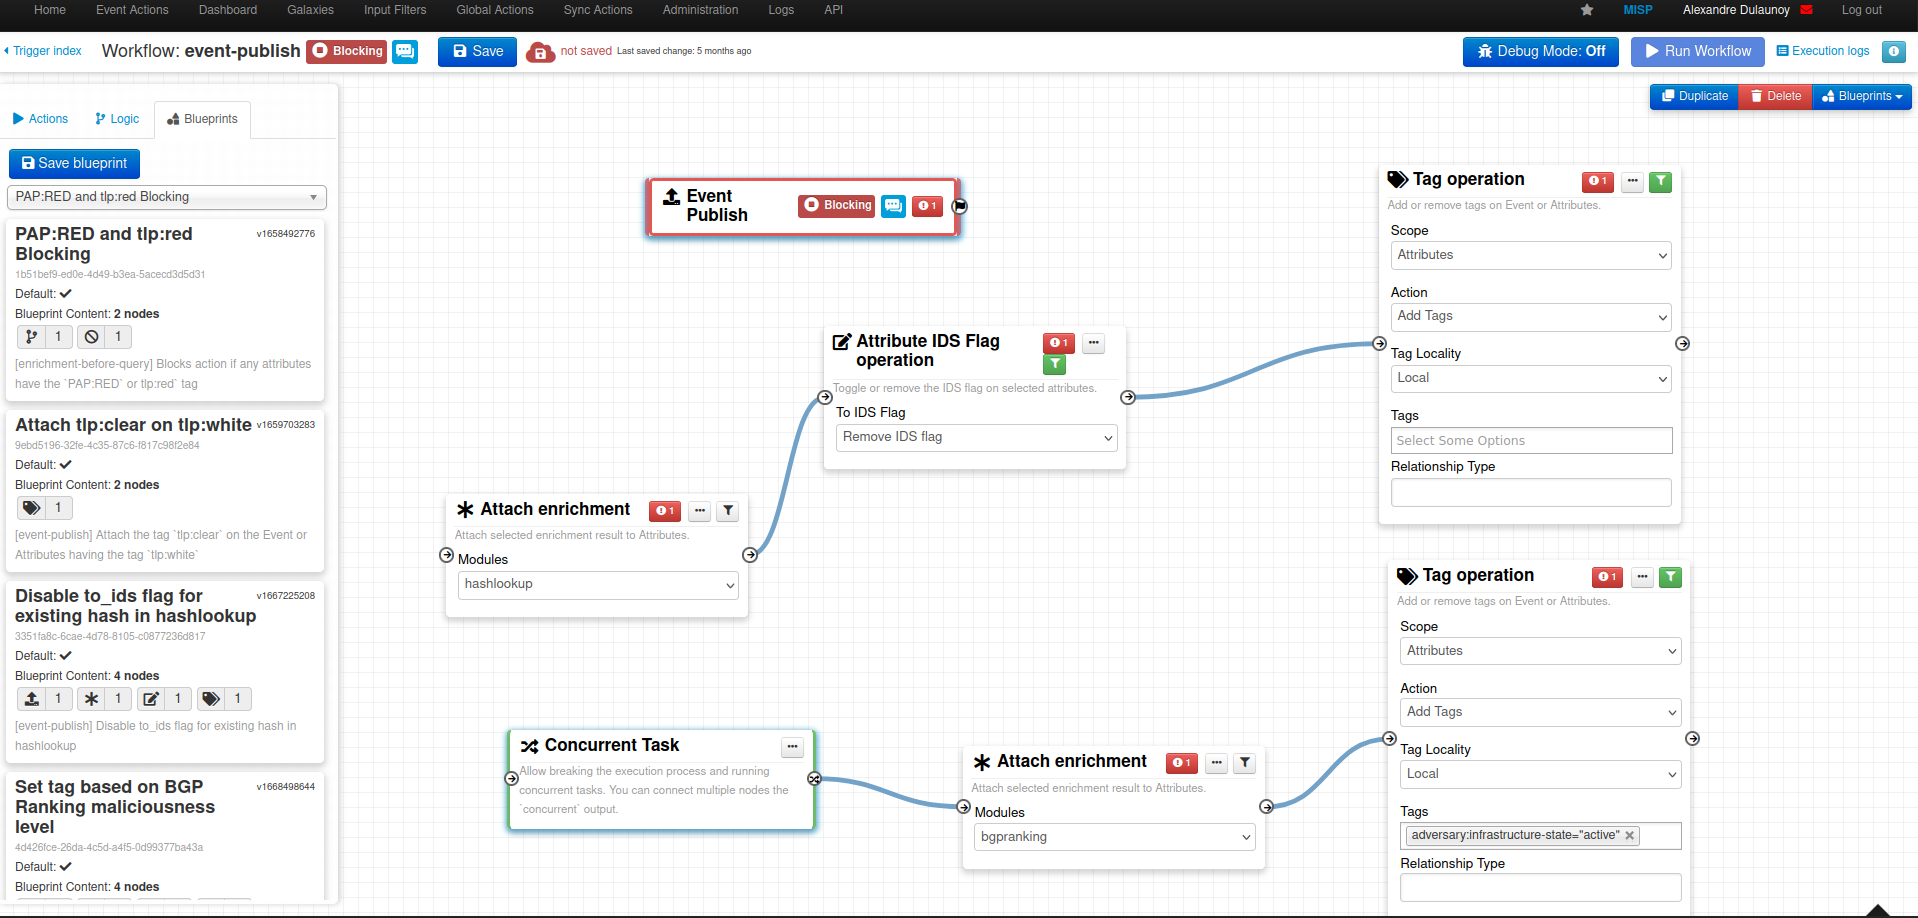
\includegraphics[scale=0.17]{images/workflows_filtered.png}
\end{center}
\end{frame}

\begin{frame}
  \frametitle{Freetext import improvements}
  \begin{itemize}
      \item The {\bf freetext import} has been a powerful way of creating {\bf attributes} parsed out of text
      \item Since 2.4.167, it can also be used to {\bf create MISP objects }
      \item {\bf Proposes} valid object {\bf templates} for the given data-points
      \item New UI elements and parsing logic added
      \item Objects in general encouraged over flat attributes
      \item Goes hand-in-hand with new {\bf object template} development
  \end{itemize}
\end{frame}

\begin{frame}
\frametitle{Freetext import improvements}
\begin{center}
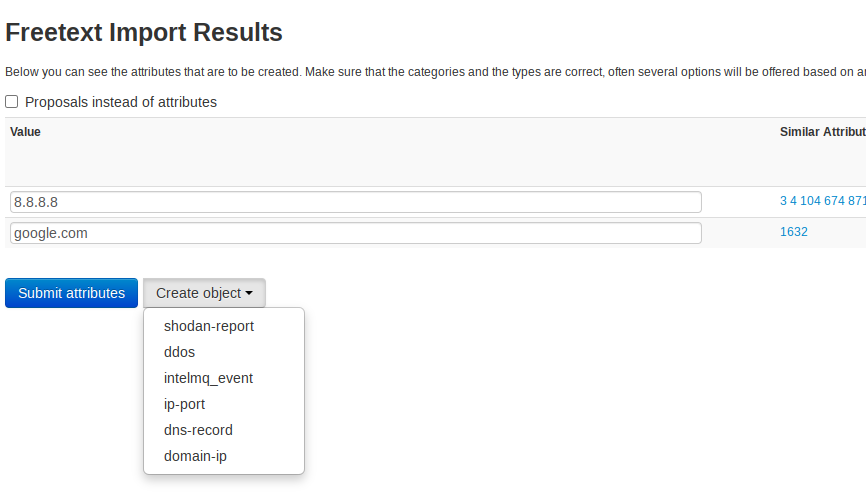
\includegraphics[scale=0.40]{images/freetext_objects.png}
\end{center}
\end{frame}


\begin{frame}
  \frametitle{Logging rework}
  \begin{itemize}
     \item {\bf Logging concerns separated} into optional separate mechanisms
     \begin{itemize}
         \item Separate Application, Audit, Access logs (thanks to Jakub Onderka)
     \end{itemize}
     \item New user sanity checks on {\bf prior authentications} and {\bf associated IPs} (thanks to Christophe Vandeplas)
     \begin{itemize}
         \item Allows users to audit their accounts' actions to catch abuse
     \end{itemize}
     \item New internal logging of {\bf authentication frequency}
  \end{itemize}
\end{frame}

\begin{frame}
  \frametitle{Dashboard rework}
  \begin{itemize}
     \item {\bf Overhaul} of the {\bf widget toolkit} for instance visibility
     \item New widgets to highlight {\bf trends, community interactions and statistics}
     \item Focus on {\bf customisation} and {\bf bucketing} of organisation groups
     \begin{itemize}
         \item Use Organisation meta-data, such as country, sector, org type
     \end{itemize}
     \item Better defined {\bf reporting periods}
     \begin{itemize}
         \item Show data of current day, month, year or since an arbitrary date
     \end{itemize}
     \item Rework of some existing widgets to be much more {\bf performant}
  \end{itemize}
\end{frame}

\begin{frame}

\frametitle{Dashboard example}
\begin{center}
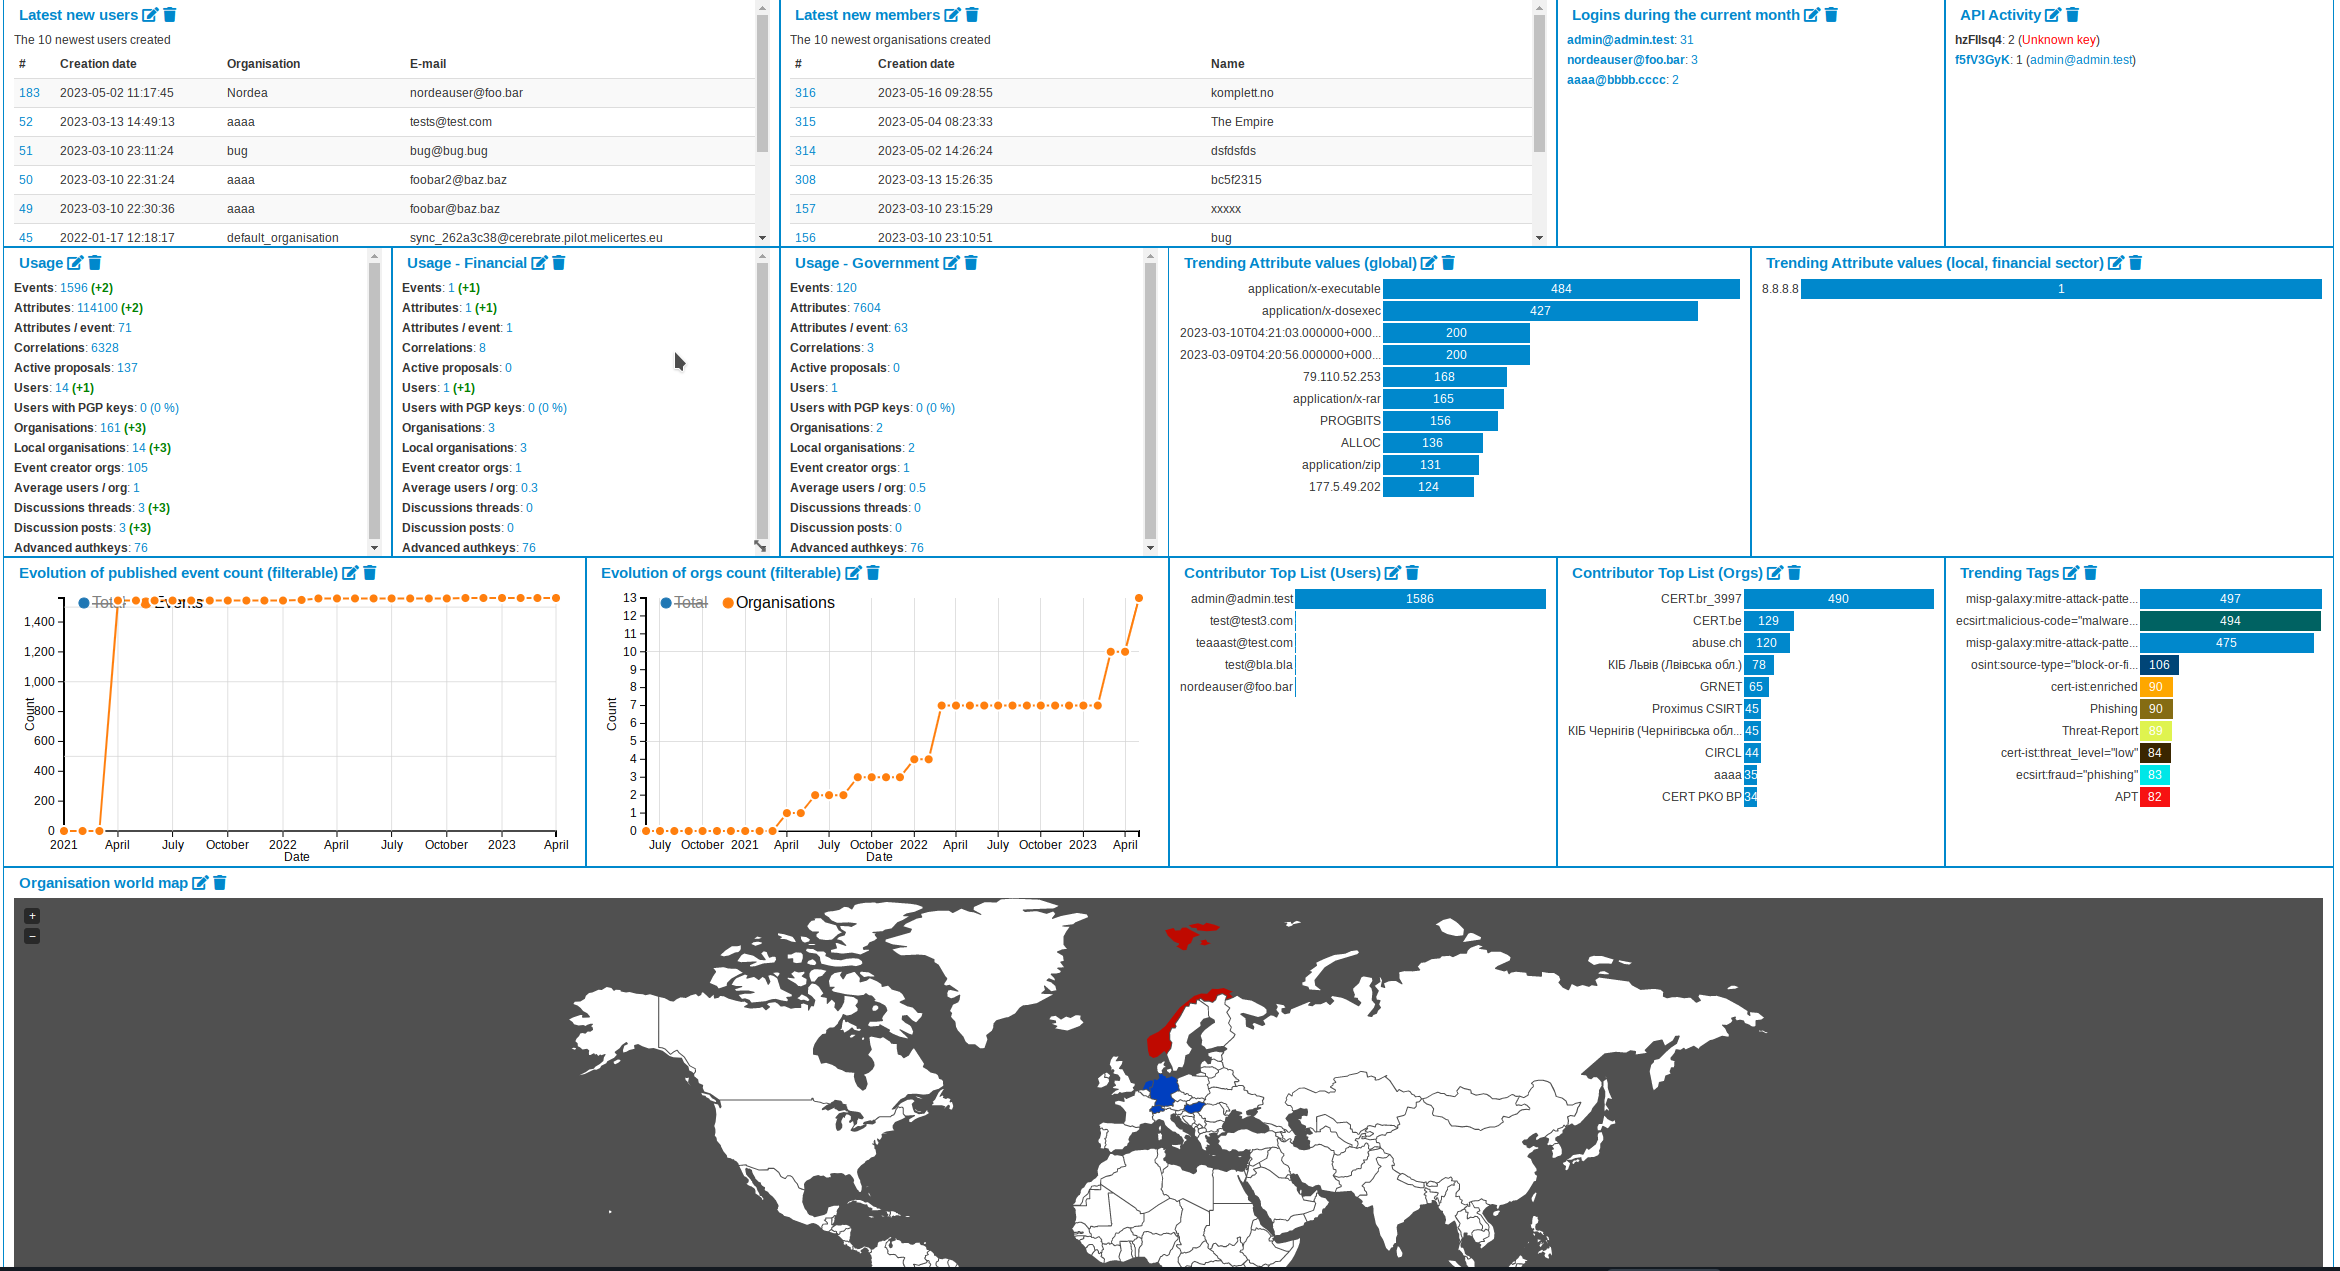
\includegraphics[scale=0.14]{images/dashboard_example.png}
\end{center}
\end{frame}

\begin{frame}
  \frametitle{Security fixes and other improvements}
  \begin{itemize}
     \item Long list of security fixes based on multiple external penetration tests
     \item {\bf CVEs}\footnote{\url{https://www.misp-project.org/security/}} continuously reported for issues small and large
     \begin{itemize}
         \item Make sure you're up to date!
     \end{itemize}
     \item {\bf Zigrin security}'s research funded by the {\bf Luxembourg army} has been a massive help
     \item Long list of other improvements, quality of life changes, performance tuning
  \end{itemize}
\end{frame}

\begin{frame}
\frametitle{Taxonomy highlight}
\begin{itemize}
    \item Many different taxonomies are used frequently in various organisations
    \item A new feature to highlight the important taxonomy in a MISP instance (community) is available
    \item Site admin user can select the {\bf highlighted taxonomies}
    \item The taxonomy namespace will be highlight in a box on the index/event views
\end{itemize}
    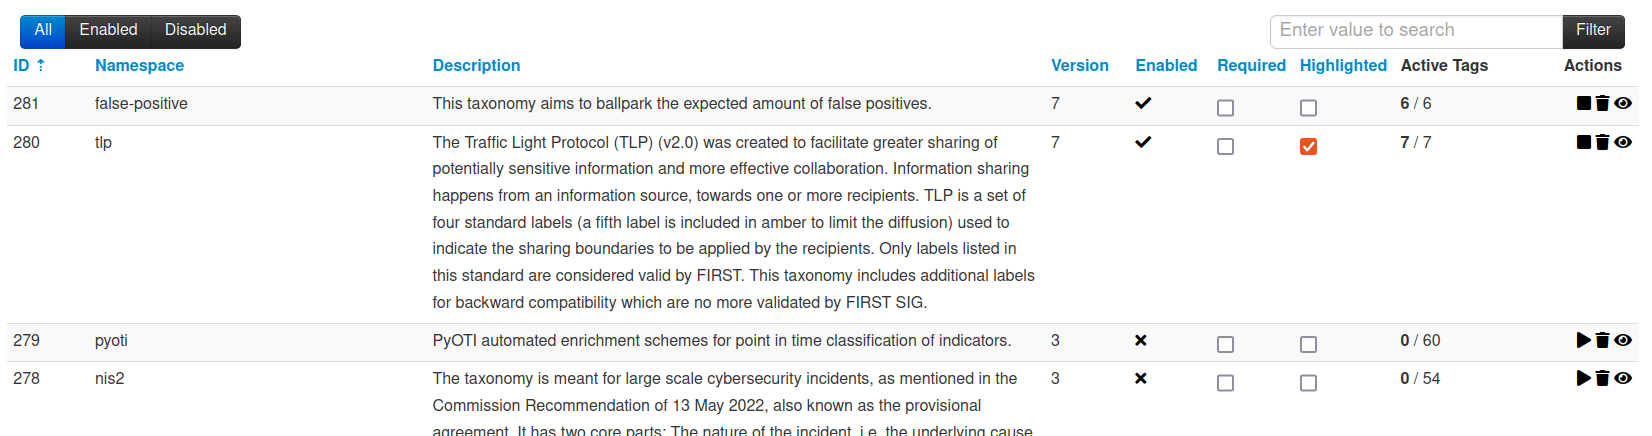
\includegraphics[scale=0.2]{./images/highlight.png}
    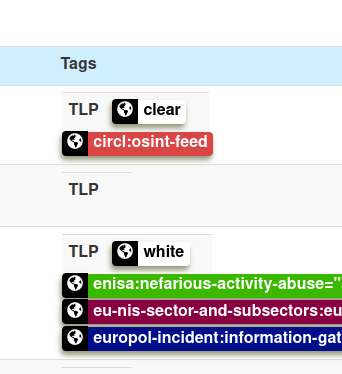
\includegraphics[scale=0.2]{./images/highlight2.png}
\end{frame}

\section{Ongoing rework}

\begin{frame}
  \frametitle{MISP 3}
  \begin{itemize}
     \item Largest ongoing work is the work on {\bf MISP3}
     \item Already announced long ago, development is now underway\footnote{\url{https://github.com/MISP/MISP/tree/3.x}}
     \item New {\bf tech stack} based on Cerebrate's advances (CakePHP 4.x+, PHP 8.2+, Bootstrap 5+)
     \item Longer project, will bring long needed improvements
  \end{itemize}
\end{frame}

\section{MISP 3 Objective}

\begin{frame}
  \frametitle{Ensuring compatibility}
  \begin{itemize}
     \item Full {\bf API compatibility} with MISP 2.4
     \item {\bf Synchronisation compatibility} with MISP 2.4
     \item At least the same {\bf feature set as MISP 2.4}
     \begin{itemize}
         \item Except for culling unused, unmaintained functionalities
         \item We are collecting usage data on CIRCL's platforms about legacy functionalities
     \end{itemize}
  \end{itemize}
\end{frame}

\begin{frame}
  \frametitle{What we expect from the upgrade process}
  \begin{itemize}
     \item The first update since 2.4 in 2015 that requires manual intervention
     \item Burden on administrators:
     \begin{itemize}
         \item We will include scripts that will install MISP3 side-by-side of MISP2 and ingest all of your MISP 2 data
         \item The process will not be automatic and will need administrator intervention
         \item Some new requirements (more modern PHP for example, new framework version's requirements)
         \item Database migration is included in the process
     \end{itemize}
     \item Versions following 3.0 will go back to a similar one-click update process for the lifecycle of 3.x
     \item This will allow us to make some changes that we've held back for too long
  \end{itemize}
\end{frame}

\begin{frame}
  \frametitle{Improvements to the database structure}
  \begin{itemize}
     \item Rework of schema for more performance
     \item Relational constraints moved to the database for consistency and performance
     \item Modernised unicode handling
     \item Fixes of some legacy mistakes (reserved keyword field use for example)
     \item DB improvements that were outcomes of research from Cerebrate incorporated (tags, metadata)
  \end{itemize}
\end{frame}

\begin{frame}
  \frametitle{Better file structure}
  \begin{itemize}
     \item Clearer separation of concerns (software codebase vs data vs logs)
     \begin{itemize}
         \item Easier containerisation of MISP
         \item Saner file permission management
         \item Simpler log collection
     \end{itemize}
     \item Reduced complexity of installation and package management
     \item Use of framework features rather than custom features for upgrade management
  \end{itemize}
\end{frame}

\begin{frame}
  \frametitle{UX rework}
  \begin{itemize}
     \item More harmonised UI
     \item Modern look and feel
     \item Easier to use interactions
     \item Menues and actions reworked to be more use-case focused
     \item UI customisation for users
  \end{itemize}
\end{frame}

\begin{frame}
\frametitle{MISP 3 UI}
\begin{center}
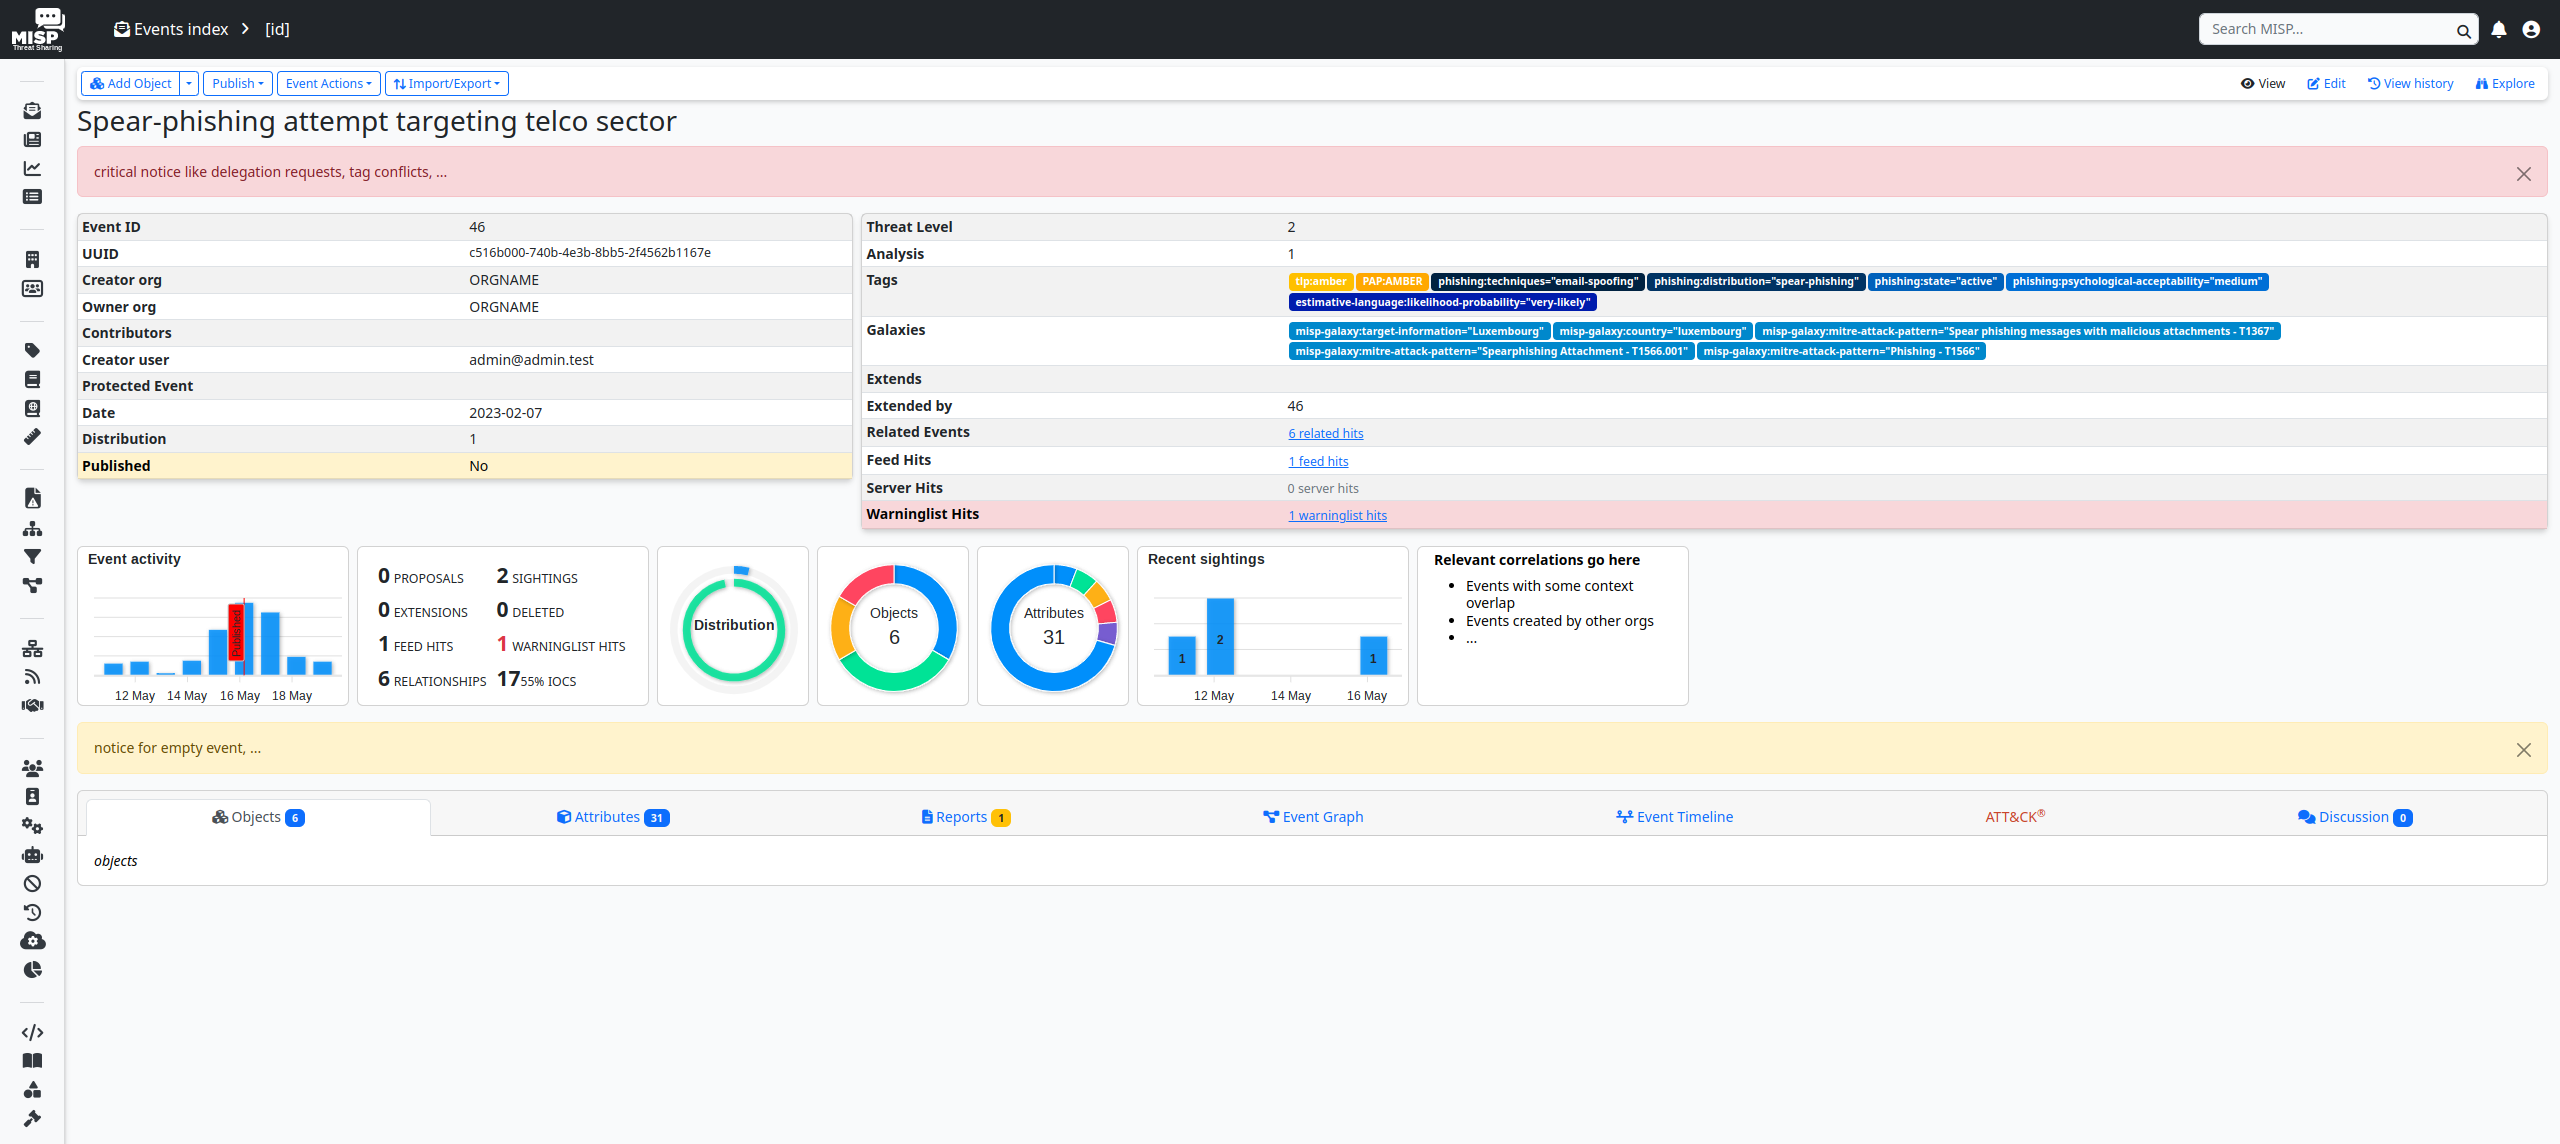
\includegraphics[scale=0.18]{images/misp3.png}
\end{center}
\end{frame}

\begin{frame}
  \frametitle{Performance tuning and software quality management}
  \begin{itemize}
     \item New framework provides better tools for performant queries
     \item New, tighter integrated testing framework used for CI
     \item The new framework version is compliant with PHP framework standards allowing us to use a wide range tools
  \end{itemize}
\end{frame}

\begin{frame}
  \frametitle{Plenty of work ahead of us to achieve our goals}
  \begin{itemize}
     \item If you, or colleagues of yours want to get involved, let us know!
     \item We're also looking for discussions on what the user-base would like to see in a reworked, modernised MISP
  \end{itemize}
\end{frame}

\section{Conclusions}

\begin{frame}
  \frametitle{To sum it all up...}
  \begin{itemize}
     \item The MISP {\bf developer community} continues to grow and stay active
     \item The main focus the past year was on the following
     \begin{itemize}
          \item Performance, security, UX improvements
          \item Customisations of workflow processes
          \item Better operationalisation of MISP (community management, integration, monitoring)
          \item Fleshing out the documentation and supporting materials
     \end{itemize}
     \item Cerebrate is aiming to fill the void of community/fleet management that we currently have
     \item Definitely no lack of new ideas and improvements, if you want to participate, it's easy to {\bf get involved}
     \item Prioritisation is hard. {\bf Let us know what you think we should focus on}!
  \end{itemize}
\end{frame}

\begin{frame}
  \frametitle{Get in touch if you have any questions}
  \begin{itemize}
    \item Contact CIRCL
    \begin{itemize}
      \item info@circl.lu
      \item \url{https://twitter.com/circl_lu}
      \item \url{https://www.circl.lu/}
    \end{itemize}
    \item Contact MISPProject 
    \begin{itemize}
      \item \url{https://github.com/MISP}
      \item \url{https://gitter.im/MISP/MISP}
      \item \url{https://twitter.com/MISPProject}
    \end{itemize}
    \item Cerebrate project
    \begin{itemize}
      \item \url{https://github.com/cerebrate-project}
      \item \url{https://github.com/cerebrate-project/cerebrate}
    \end{itemize}
  \end{itemize}
\end{frame}
